\xiti
\begin{xiaotis}

\xiaoti{把下列命题写成 “如果…,那么…” 的形式:}
\begin{xiaoxiaotis}

    \xxt{两条平行线被第三条直线所截,同旁内角互补;}

    \xxt{直角都相等。}

\end{xiaoxiaotis}


抄下列各题,并在括号内加注理由和填空:

\xiaoti{如图,已知:$\angle A + \angle B = 180^\circ$。\\
    求证: $\angle C + \angle D = 180^\circ$。 \\
    \zhengming $\because$ \quad $\angle A + \angle B = 180^\circ$ (\hspace*{2cm}), \\
    $\therefore$ \quad $AD \pingxing BC$ (\hspace*{2cm})。 \\
    $\therefore$ \quad $\angle C + \angle D = 180^\circ$ (\hspace*{2cm})。
}

\begin{figure}[htbp]
    \centering
    \begin{minipage}[b]{7cm}
        \centering
        \begin{tikzpicture}
    \tkzDefPoints{0/0/B, 4/0/C,  1/2/A,  3.5/2/D}

    \tkzDrawPolygon(A,B,C,D)
    \tkzLabelPoints[below](B,C)
    \tkzLabelPoints[above](A,D)
\end{tikzpicture}


        \caption*{(第 2 题)}
    \end{minipage}
    \qquad
    \begin{minipage}[b]{7cm}
        \centering
        \begin{tikzpicture}
    \tkzDefPoints{0/0/C, 4/0/D,  2/2/A,  2/0/B}

    \tkzDrawSegments(A,B  C,D)
    \tkzMarkRightAngles[size=0.3](A,B,C  D,B,A)
    \tkzLabelAngle[pos=0.7](A,B,C){$1$}
    \tkzLabelAngle[pos=0.7](D,B,A){$2$}
    \tkzLabelPoints[below](B,C,D)
    \tkzLabelPoints[right](A)
\end{tikzpicture}


        \caption*{(第 3 题)}
    \end{minipage}
\end{figure}

\xiaoti{已知:$AB \perp CD$。\\
    求证: $\angle 1 = \angle 2$。 \\
    \zhengming $\because$ \quad $AB \perp CD$ (\hspace*{2cm}), \\
    $\therefore$ \quad $\angle 1 = 90^\circ$, $\angle 2 = 90^\circ$ (\hspace*{2cm})。 \\
    $\therefore$ \quad $\angle 1 = \angle 2$ (\hspace*{2cm})。
}



\xiaoti{已知:$AB \pingxing CD$,$BC \pingxing DE$。\\
    求证: $\angle B + \angle D = 180^\circ$。 \\
    \zhengming $\because$ \quad $AB \pingxing CD$ (\hspace*{2cm}), \\
    $\therefore$ \quad $\angle B = \text{(\hspace*{1cm})}$ (\hspace*{2cm})。 \\
    $\because$ \quad $BC \pingxing \text{(\hspace*{1cm})}$ (\hspace*{2cm}), \\
    $\therefore$ \quad $\angle C + \angle D = 180^\circ$ (\hspace*{2cm})。 \\
    $\therefore$ \quad $\angle B + \angle D = 180^\circ$ (\hspace*{2cm})。
}

\begin{figure}[htbp]
    \centering
    \begin{minipage}[b]{7cm}
        \centering
        \begin{tikzpicture}
    \tkzDefPoints{0/0/C, 2/0/D,  1/3/B,  3/3/E, -1/3/A}

    \tkzDrawSegments(A,B  B,C  C,D  D,E)
    \tkzLabelPoints[below](A)
    \tkzLabelPoints[left](C)
    \tkzLabelPoints[right](B,D,E)
\end{tikzpicture}


        \caption*{(第 4 题)}
    \end{minipage}
    \qquad
    \begin{minipage}[b]{7cm}
        \centering
        \begin{tikzpicture}
    \tkzDefPoints{0/0/A, 4/0/B,  1/3/D,  5/3/C}

    \tkzDrawPolygon(A,B,C,D)
    \tkzDrawSegments(A,C)
    \tkzMarkAngles[size=0.3](C,A,D  A,C,B)
    \tkzMarkAngles[size=0.5](B,A,C  D,C,A)
    \tkzLabelAngle[pos=0.5](C,A,D){$1$}
    \tkzLabelAngle[pos=0.5](A,C,B){$2$}
    \tkzLabelAngle[pos=0.7](B,A,C){$3$}
    \tkzLabelAngle[pos=0.7](D,C,A){$4$}
    \tkzLabelPoints[below](A,B)
    \tkzLabelPoints[above](C,D)
\end{tikzpicture}


        \caption*{(第 5 题)}
    \end{minipage}
\end{figure}


\xiaoti{已知:$AD \pingxing BC$,$\angle BAD = \angle BCD$。\\
    求证: $AB \pingxing CD$。 \\
    \zhengming $\because$ \quad $AD \pingxing BC$ (\hspace*{2cm}), \\
    $\therefore$ \quad $\angle 1 = \text{(\hspace*{1cm})}$ (\hspace*{2cm})。 \\
    又$\because$ \quad $\angle BAD = \angle BCD$ (\hspace*{2cm}), \\
    $\therefore$ \quad $\angle BAD - \angle 1 = \angle BCD - \angle 2$ (\hspace*{2cm})。 \\
    即 \quad $\angle 3 = \angle 4$。 \\
    $\therefore$ \quad $AB \pingxing \text{(\hspace*{1cm})}$ (\hspace*{2cm})。
}


\begin{enhancedline}
\xiaoti{已知: $AB \pingxing CD$, $AE$、$DF$ 分别是 $\angle BAD$、$\angle CDA$ 的角平分线。\\
    求证: $AE \pingxing DF$。 \\
    \zhengming $\because$ \quad $AB \pingxing CD$ (\hspace*{2cm}), \\
    $\therefore$ \quad $\angle BAD = \text{(\hspace*{1cm})}$ (\hspace*{2cm})。 \\
    $\because$ \quad $AE$、$DF$ 分别是 $\angle BAD$、$\angle CDA$ 的角平分线 (\hspace*{2cm}), \\
    $\therefore$ \quad $\angle 1 = \exdfrac{1}{2} \angle BAD$, $\angle 2 = \exdfrac{1}{2} \angle CDA$ (\hspace*{2cm})。 \\
    $\therefore$ \quad $\angle 1 = \angle 2$ (\hspace*{2cm})。 \\
    $\therefore$ \quad $AE \pingxing \text{(\hspace*{1cm})}$ (\hspace*{2cm})。
}
\end{enhancedline}

\begin{figure}[htbp]
    \centering
    \begin{minipage}[b]{7cm}
        \centering
        \begin{tikzpicture}
    \tkzDefPoints{0/0/C, 3/0/D,  1/3/A,  4/3/B}
    \tkzDefLine[bisector](D,A,B) \tkzGetPoint{E}
    \tkzDefLine[bisector](A,D,C) \tkzGetPoint{F}

    \tkzDrawSegments(C,D  D,A  A,B)
    \tkzDrawSegments(A,E  D,F)
    \tkzMarkAngles[size=0.6](D,A,E  A,D,F)
    \tkzLabelAngle[pos=0.9](D,A,E){$1$}
    \tkzLabelAngle[pos=0.9](A,D,F){$2$}
    \tkzLabelPoints[below](C,D,F)
    \tkzLabelPoints[above](A,B)
    \tkzLabelPoints[right](E)
\end{tikzpicture}


        \caption*{(第 6 题)}
    \end{minipage}
    \qquad
    \begin{minipage}[b]{7cm}
        \centering
        \begin{tikzpicture}
    \tkzDefPoints{0/0/E, 3/0/F, -0.5/1/C,  3/1/D, -1.5/3/A,  3/3/B}

    \tkzDrawSegments(A,B  C,D  E,F  A,E)
    \tkzMarkAngles[size=0.4](E,A,B)
    \tkzMarkAngles[size=0.5](D,C,A)
    \tkzLabelAngle[pos=0.6](E,A,B){$1$}
    \tkzLabelAngle[pos=0.8](D,C,A){$2$}
    \tkzLabelPoints[left](A,C,E)
    \tkzLabelPoints[right](B,D,F)
\end{tikzpicture}


        \caption*{(第 7 题)}
    \end{minipage}
\end{figure}


\xiaoti{已知: $AB \pingxing EF$, $\angle 1 + \angle 2 = 180^\circ$。\\
    求证: $CD \pingxing EF$。 \\
    \zhengming $\because$ \quad $\angle 1 + \angle 2 = 180^\circ$ (\hspace*{2cm}), \\
    $\therefore$ \quad $AB \pingxing \text{(\hspace*{1cm})}$ (\hspace*{2cm})。 \\
    又 $\because$ \quad $\text{(\hspace*{1cm})} \pingxing EF$ (\hspace*{2cm}), \\
    $\therefore$ \quad $CD \pingxing EF$ (\hspace*{2cm})。
}


\xiaoti{证明下列命题是假命题:}
\begin{xiaoxiaotis}

    \xxt{如果一个数能被 2 整除,那么这个数也能被 4 整除;}

    \xxt{不等式的两边都乘以同一个数,不等号的方向不变;}

    \xxt{一个锐角与一个钝角的和等于一个平角。}

\end{xiaoxiaotis}


\xiaoti{画图,并写出已知、求证(不证明):}
\begin{xiaoxiaotis}

    \xxt{同角的补角相等;}

    \xxt{邻补角的平分线互相垂直;}

    \xxt{对顶角的平分线成一条直线。}

\end{xiaoxiaotis}

\end{xiaotis}

